\documentclass[tikz,border=5pt]{standalone}
\usepackage{amsmath,amssymb}
\usetikzlibrary{arrows.meta,positioning,calc}
\begin{document}
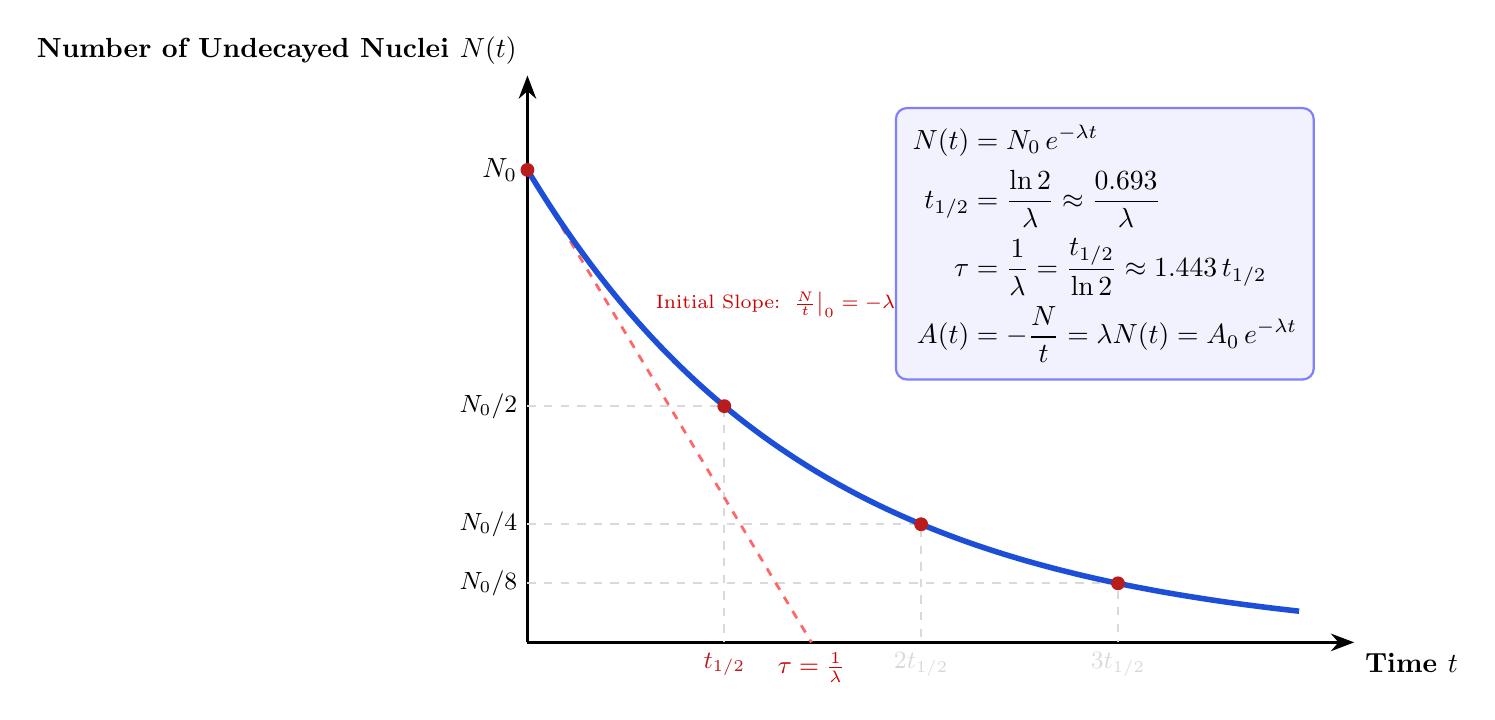
\begin{tikzpicture}[>=Stealth, font=\sffamily, thick]
  \definecolor{decayblue}{HTML}{1D4ED8}
  \definecolor{hlred}{HTML}{B91C1C}

  % Axes
  \draw[->, line width=1.2pt] (0,0) -- (10.5,0) node[below right, font=\bfseries] {Time $t$};
  \draw[->, line width=1.2pt] (0,0) -- (0,7.2) node[above left, font=\bfseries] {Number of Undecayed Nuclei $N(t)$};

  % Ticks & grid
  \node[left, font=\bfseries] at (0,6.0) {$N_0$};
  \node[left, font=\small] at (0,3.0) {$N_0 / 2$};
  \node[left, font=\small] at (0,1.5) {$N_0 / 4$};
  \node[left, font=\small] at (0,0.75) {$N_0 / 8$};

  \draw[gray!30, dashed] (0,3.0) -- (2.5,3.0) -- (2.5,0) node[below, font=\bfseries\small, text=hlred] {$t_{1/2}$};
  \draw[gray!30, dashed] (0,1.5) -- (5.0,1.5) -- (5.0,0) node[below, font=\small] {$2t_{1/2}$};
  \draw[gray!30, dashed] (0,0.75) -- (7.5,0.75) -- (7.5,0) node[below, font=\small] {$3t_{1/2}$};

  % Tangent at t=0
  \draw[red!60, line width=1pt, dashed] (0,6.0) -- (3.6067, 0) node[below, text=red!80!black, font=\bfseries\small] {$\tau = \frac{1}{\lambda}$};
  \node[above right, text=red!80!black, font=\scriptsize] at (1.5, 4.0) {Initial Slope: $\left.\frac{\dd N}{\dd t}\right|_0 = -\lambda N_0$};

  % Exponential decay curve
  \draw[line width=2pt, decayblue, domain=0:9.8, samples=100]
    plot (\x, {6.0 * exp(-0.27725887 * \x)});

  % Key points
  \fill[hlred] (0,6.0) circle (2.5pt);
  \fill[hlred] (2.5,3.0) circle (2.5pt);
  \fill[hlred] (5.0,1.5) circle (2.5pt);
  \fill[hlred] (7.5,0.75) circle (2.5pt);

  % Formula box
  \node[draw=blue!50, fill=blue!5, rounded corners=4pt, inner sep=6pt, anchor=north east] at (10.0,6.8) {
    $\begin{aligned}
      N(t) &= N_0\,e^{-\lambda t} \\
      t_{1/2} &= \frac{\ln 2}{\lambda} \approx \frac{0.693}{\lambda} \\
      \tau &= \frac{1}{\lambda} = \frac{t_{1/2}}{\ln 2} \approx 1.443\,t_{1/2} \\
      A(t) &= -\frac{\dd N}{\dd t} = \lambda N(t) = A_0\,e^{-\lambda t}
    \end{aligned}$
  };
\end{tikzpicture}
\end{document}
